Last time, we discovered the mildly disturbing fact that our bosonic string theory has tachyons. Having made note of this, we decided to take it on faith that superstring theory has a reasonable solution to this problem, and proceeded to define massless modes of the string by
\begin{align}
    \ket{g} &= h_{\mu\nu} \alpha_{-1}^{(\mu} \bar \alpha_{-1}^{\nu)} \ket{k}\\
    \ket{B} &= B_{\mu\nu} \alpha_{-1}^{[\mu} \bar \alpha_{-1}^{\nu]} \ket{k}\\
    \ket{\phi}&=\phi \alpha_{-1}^\mu \bar \alpha_{-1 \mu} \ket{k}.
\end{align}

These correspond sort of to a graviton ($g_{\mu\nu}=\eta_{\mu\nu}+h_{\mu\nu}$), a $B$-field (since $B_{\mu\nu}=-B_{\nu\mu}$), and a so-called dilaton $\phi$ (scalar field). One can show that these fields arise as a linear approximation to the theory described by the following spacetime action:
\begin{equation}
    S=-\frac{1}{2K^2} \int d^Dx \sqrt{-g}e^{-2\phi}\paren{
        R-4\p_\mu \phi \p^\mu \phi +\frac{1}{12} H_{\mu\nu\lambda} H^{\mu\nu\lambda}
        },
\end{equation}
where $H_{\mu\nu\lambda}=\p_{[\mu}B_{\nu\lambda]}$ and $K$ is a coupling constant which will be related to Newton's gravitational constant in $D$ dimensions.

This suggests to us that the fields and modes on our worldsheet have in fact told us something about how to deform the background (until now Minkowski) metric, so we could consider the more general starting point
\begin{equation}
    S_1[X,h]=-\frac{1}{4\pi \alpha'} \int_\Sigma d^2\sigma \sqrt{-h}h^{ab} \p_a X^ \mu \p_b X^\nu g_{\mu\nu}(X).
\end{equation}

Moreover, it turns out that the quantum theory has Weyl symmetry if $g_{\mu\nu}(x)$ satisfies
\begin{equation*}
    R_{\mu\nu}=0
\end{equation*}
to first order in $\alpha'$ (the only parameter in our theory, really), which are simply the Einstein equations in vacuum. That is, imposing the symmetry of the quantum theory on the worldsheet results in a condition on the background metric in all of spacetime. Higher orders will give corrections to this result -- to next order in $\alpha'$, 
\begin{equation}
    R_{\mu\nu}+\frac{\alpha'}{2} R_{\mu\rho\lambda\sigma} R_{\nu}^{\rho\lambda\sigma}=0.
\end{equation}
Our theory therefore suggests that there are higher order corrections to the Einstein equations.

We could also add a term like
\begin{equation}
    S_2=-\frac{1}{4\pi \alpha'} \int_\Sigma d^2\sigma \sqrt{-h} \epsilon^{ab} \p_a X^\mu \p_b X^\nu B_{\mu\nu},
\end{equation}
with $\epsilon^{ab}$ the completely antisymmetric rank two tensor. This links the action to the stress-energy tensor of our $B$-field.

Finally, we could add a coupling to the dilaton,
\begin{equation}
    S_3=\frac{1}{4\pi} \int_\Sigma d^2\sigma \sqrt{-h} \phi(X) R_\Sigma,
\end{equation}
with $R_\Sigma$ the worldsheet Ricci scalar.

The condition that the action
\begin{equation*}
    S=S_1+S_2+S_3
\end{equation*}
gives a Weyl-invariant quantum theory results in what we might call equations of motion in spacetime for $g_{\mu\nu},B_{\mu\nu},$ and $\phi.$ To leading order in $\alpha'$, these equations of motion may be derived from the action
\begin{equation*}
    S=-\frac{1}{2K^2} \int d^Dx \sqrt{-g}e^{-2\phi}\paren{
        R-4\p_\mu \phi \p^\mu \phi +\frac{1}{12} H_{\mu\nu\lambda} H^{\mu\nu\lambda}
        }+O(\alpha').
\end{equation*}
If you like, the worldsheet theory couples to the metric of the background spacetime. Now, we could have just written down this action to start with. But deriving it from the worldsheet allows us to argue that any higher order terms are suppressed by the length scale of $\alpha'$.

What happens if spacetime has some weird topology? Consider a theory where spacetime has the topology of $\RR^2\times S^1$, as in Fig. \ref{fig:stringtopology}
\begin{figure}
    \centering
    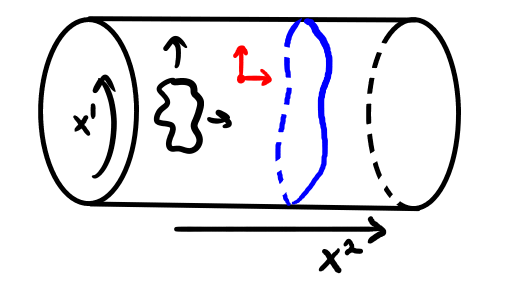
\includegraphics[width=0.5\textwidth]{2019/01/20190130_stringtopology.png}
    \caption{A spacetime with the topology $\RR^2\times S^1$. A particle (red) can move along the length of the cylinder and around its circumference. A string on the surface (black) can do the same. But this spacetime also admits the string configuration (blue) which wraps around the circumference.}
    \label{fig:stringtopology}
\end{figure}
Then a string can move around the spacetime just like a particle, but it can also wrap around the compact $S^1$ direction and probe the topology of the spacetime. Therefore something else interesting is happening which the modes we've currently defined seem totally insensitive to.

\subsection*{Path integral quantization}
Some of the details of path integral quantization are covered in \emph{Advanced Quantum Field Theory}, and also in Polchinski (appendix in vol. 1), as well as in Ryder on QFT and Feynman and Hibbs (though this last one is broadly maligned for having errors in other sections).

Path integrals give us a conceptually different way to think about calculating amplitudes in QM and more generally in QFT. Morally speaking, a path integral is a weighted sum of paths satisfying some boundary conditions,
\begin{equation}
    \braket{x_f,t_t}{x_i,t_i}=\int_{x(t_i)}^{x(t_f)} \cD x e^{iS[x]}
\end{equation}
for some action $S[x]=\int_{t_i}^{t_f} dt L (x,\dot x)$. We will be interested in the apath integral quantization of the Polyakov action.

That is, given some initial and final string states $\Psi_{i,f}$, the path integral is
\begin{equation}
    \braket{\Psi_f}{\Psi_i}=\int_i^f \cD x \cD h e^{iS[h,x]},
\end{equation}
with $S[h,x]$ the Polyakov action. But now by analogy with QFT we will have to deal with strings splitting and merging in our path integral, as shown in Fig. \ref{fig:stringpathintegral}. There will be new complications when we try to compute the path integral.

\begin{figure}
    \centering
    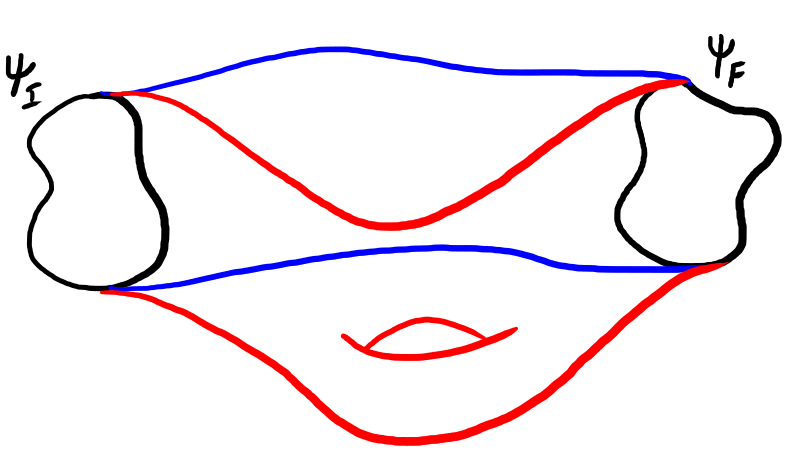
\includegraphics[width=0.5\textwidth]{2019/01/20190130_stringpathintegral.png}
    \caption{Two worldsheet configurations we might need to sum over in the path integral from $\Psi_i$ (left) to $\Psi_f$ (right). One worldsheet (blue) has the string propagating directly from $\Psi_i$ to $\Psi_f$, while the other (red) has the string pinching off and splitting into two before merging back (the equivalent of a scattering process in QFT).}
    \label{fig:stringpathintegral}
\end{figure}